


\tikzset{every picture/.style={line width=0.75pt}} %set default line width to 0.75pt        

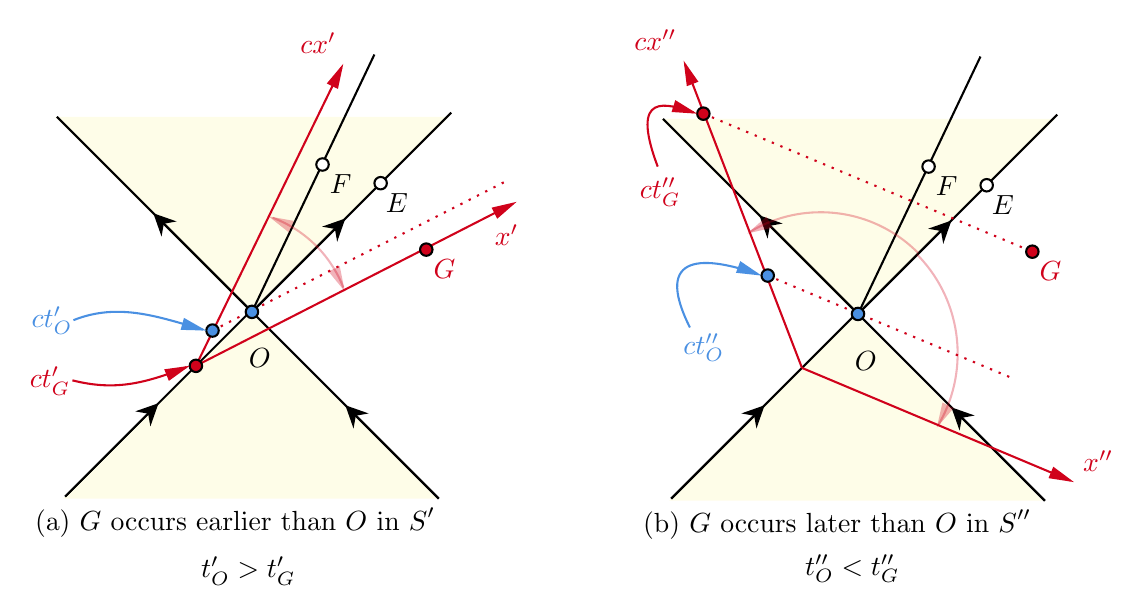
\begin{tikzpicture}[x=0.75pt,y=0.75pt,yscale=-1,xscale=1]
%uncomment if require: \path (0,288); %set diagram left start at 0, and has height of 288

%Shape: Triangle [id:dp9951602844722451] 
\draw  [draw opacity=0][fill={rgb, 255:red, 248; green, 231; blue, 28 }  ,fill opacity=0.1 ] (138,147) -- (228,237) -- (48,237) -- cycle ;
%Shape: Triangle [id:dp859629594586236] 
\draw  [draw opacity=0][fill={rgb, 255:red, 248; green, 231; blue, 28 }  ,fill opacity=0.1 ] (138,147) -- (234,53) -- (44,53) -- cycle ;
%Straight Lines [id:da473248405361371] 
\draw [color={rgb, 255:red, 0; green, 0; blue, 0 }  ,draw opacity=1 ]   (139,146) -- (49,236) ;
%Straight Lines [id:da762095141309328] 
\draw [color={rgb, 255:red, 0; green, 0; blue, 0 }  ,draw opacity=1 ]   (45,53) -- (139,147) ;
%Straight Lines [id:da23643130377054677] 
\draw [color={rgb, 255:red, 0; green, 0; blue, 0 }  ,draw opacity=1 ]   (139,147) -- (235,51) ;
%Straight Lines [id:da0519512830410056] 
\draw [color={rgb, 255:red, 0; green, 0; blue, 0 }  ,draw opacity=1 ]   (139,147) -- (229,237) ;
%Straight Lines [id:da8809453026912568] 
\draw [color={rgb, 255:red, 0; green, 0; blue, 0 }  ,draw opacity=1 ]   (49,236) -- (91.88,193.12) ;
\draw [shift={(94,191)}, rotate = 135] [fill={rgb, 255:red, 0; green, 0; blue, 0 }  ,fill opacity=1 ][line width=0.08]  [draw opacity=0] (10.72,-5.15) -- (0,0) -- (10.72,5.15) -- (7.12,0) -- cycle    ;
%Straight Lines [id:da8892271590541299] 
\draw [color={rgb, 255:red, 0; green, 0; blue, 0 }  ,draw opacity=1 ]   (139,147) -- (93.62,101.62) ;
\draw [shift={(91.5,99.5)}, rotate = 45] [fill={rgb, 255:red, 0; green, 0; blue, 0 }  ,fill opacity=1 ][line width=0.08]  [draw opacity=0] (10.72,-5.15) -- (0,0) -- (10.72,5.15) -- (7.12,0) -- cycle    ;
%Straight Lines [id:da08491350319878221] 
\draw [color={rgb, 255:red, 0; green, 0; blue, 0 }  ,draw opacity=1 ]   (139,147) -- (181.88,104.12) ;
\draw [shift={(184,102)}, rotate = 135] [fill={rgb, 255:red, 0; green, 0; blue, 0 }  ,fill opacity=1 ][line width=0.08]  [draw opacity=0] (10.72,-5.15) -- (0,0) -- (10.72,5.15) -- (7.12,0) -- cycle    ;
%Straight Lines [id:da4137739687974715] 
\draw [color={rgb, 255:red, 0; green, 0; blue, 0 }  ,draw opacity=1 ]   (139,147) -- (198,23) ;
%Shape: Circle [id:dp5320765918148054] 
\draw  [color={rgb, 255:red, 0; green, 0; blue, 0 }  ,draw opacity=1 ][fill={rgb, 255:red, 255; green, 255; blue, 255 }  ,fill opacity=1 ] (170,76) .. controls (170,74.34) and (171.34,73) .. (173,73) .. controls (174.66,73) and (176,74.34) .. (176,76) .. controls (176,77.66) and (174.66,79) .. (173,79) .. controls (171.34,79) and (170,77.66) .. (170,76) -- cycle ;
%Shape: Circle [id:dp1413463083809572] 
\draw  [color={rgb, 255:red, 0; green, 0; blue, 0 }  ,draw opacity=1 ][fill={rgb, 255:red, 255; green, 255; blue, 255 }  ,fill opacity=1 ] (198,85) .. controls (198,83.34) and (199.34,82) .. (201,82) .. controls (202.66,82) and (204,83.34) .. (204,85) .. controls (204,86.66) and (202.66,88) .. (201,88) .. controls (199.34,88) and (198,86.66) .. (198,85) -- cycle ;
%Straight Lines [id:da7384361108181441] 
\draw [color={rgb, 255:red, 0; green, 0; blue, 0 }  ,draw opacity=1 ]   (229,237) -- (186.12,194.12) ;
\draw [shift={(184,192)}, rotate = 45] [fill={rgb, 255:red, 0; green, 0; blue, 0 }  ,fill opacity=1 ][line width=0.08]  [draw opacity=0] (10.72,-5.15) -- (0,0) -- (10.72,5.15) -- (7.12,0) -- cycle    ;
%Straight Lines [id:da09997135433256732] 
\draw [color={rgb, 255:red, 208; green, 2; blue, 27 }  ,draw opacity=1 ]   (112,173) -- (264.72,94.91) ;
\draw [shift={(266.5,94)}, rotate = 152.92] [fill={rgb, 255:red, 208; green, 2; blue, 27 }  ,fill opacity=1 ][line width=0.08]  [draw opacity=0] (12,-3) -- (0,0) -- (12,3) -- cycle    ;
%Straight Lines [id:da8187089511396088] 
\draw [color={rgb, 255:red, 208; green, 2; blue, 27 }  ,draw opacity=1 ]   (112,173) -- (182.12,29.3) ;
\draw [shift={(183,27.5)}, rotate = 116.01] [fill={rgb, 255:red, 208; green, 2; blue, 27 }  ,fill opacity=1 ][line width=0.08]  [draw opacity=0] (12,-3) -- (0,0) -- (12,3) -- cycle    ;
%Shape: Circle [id:dp5730617468745536] 
\draw  [color={rgb, 255:red, 0; green, 0; blue, 0 }  ,draw opacity=1 ][fill={rgb, 255:red, 208; green, 2; blue, 27 }  ,fill opacity=1 ] (220,117) .. controls (220,115.34) and (221.34,114) .. (223,114) .. controls (224.66,114) and (226,115.34) .. (226,117) .. controls (226,118.66) and (224.66,120) .. (223,120) .. controls (221.34,120) and (220,118.66) .. (220,117) -- cycle ;
%Shape: Arc [id:dp36250914630275455] 
\draw  [draw opacity=0][line width=0.75]  (170.21,115.44) .. controls (176.18,121.52) and (180.84,128.89) .. (183.72,137.1) -- (128.49,156.47) -- cycle ; \draw [color={rgb, 255:red, 208; green, 2; blue, 27 }  ,draw opacity=0.3 ][line width=0.75]    (170.21,115.44) .. controls (175.73,121.06) and (180.13,127.79) .. (183.04,135.26) ; \draw [shift={(183.72,137.1)}, rotate = 244.66] [fill={rgb, 255:red, 208; green, 2; blue, 27 }  ,fill opacity=0.3 ][line width=0.08]  [draw opacity=0] (12,-3) -- (0,0) -- (12,3) -- cycle    ; 
%Straight Lines [id:da6405832767022184] 
\draw [color={rgb, 255:red, 208; green, 2; blue, 27 }  ,draw opacity=1 ][line width=0.75]  [dash pattern={on 0.84pt off 2.51pt}]  (120,156) -- (261.5,84) ;
%Shape: Circle [id:dp745400919568012] 
\draw  [color={rgb, 255:red, 0; green, 0; blue, 0 }  ,draw opacity=1 ][fill={rgb, 255:red, 74; green, 144; blue, 226 }  ,fill opacity=1 ] (136,147) .. controls (136,145.34) and (137.34,144) .. (139,144) .. controls (140.66,144) and (142,145.34) .. (142,147) .. controls (142,148.66) and (140.66,150) .. (139,150) .. controls (137.34,150) and (136,148.66) .. (136,147) -- cycle ;
%Shape: Circle [id:dp46445613158230725] 
\draw  [color={rgb, 255:red, 0; green, 0; blue, 0 }  ,draw opacity=1 ][fill={rgb, 255:red, 74; green, 144; blue, 226 }  ,fill opacity=1 ] (117,156) .. controls (117,154.34) and (118.34,153) .. (120,153) .. controls (121.66,153) and (123,154.34) .. (123,156) .. controls (123,157.66) and (121.66,159) .. (120,159) .. controls (118.34,159) and (117,157.66) .. (117,156) -- cycle ;
%Shape: Circle [id:dp4140888015788111] 
\draw  [color={rgb, 255:red, 0; green, 0; blue, 0 }  ,draw opacity=1 ][fill={rgb, 255:red, 208; green, 2; blue, 27 }  ,fill opacity=1 ] (109,173) .. controls (109,171.34) and (110.34,170) .. (112,170) .. controls (113.66,170) and (115,171.34) .. (115,173) .. controls (115,174.66) and (113.66,176) .. (112,176) .. controls (110.34,176) and (109,174.66) .. (109,173) -- cycle ;
%Curve Lines [id:da16494693927024828] 
\draw [color={rgb, 255:red, 74; green, 144; blue, 226 }  ,draw opacity=1 ]   (53,151) .. controls (74.94,142.23) and (94.5,149.61) .. (115.39,155.55) ;
\draw [shift={(117,156)}, rotate = 195.59] [fill={rgb, 255:red, 74; green, 144; blue, 226 }  ,fill opacity=1 ][line width=0.08]  [draw opacity=0] (12,-3) -- (0,0) -- (12,3) -- cycle    ;
%Curve Lines [id:da2841812413979963] 
\draw [color={rgb, 255:red, 208; green, 2; blue, 27 }  ,draw opacity=1 ]   (52.5,180) .. controls (72,184.88) and (85.8,182.15) .. (107.33,173.66) ;
\draw [shift={(109,173)}, rotate = 158.2] [fill={rgb, 255:red, 208; green, 2; blue, 27 }  ,fill opacity=1 ][line width=0.08]  [draw opacity=0] (12,-3) -- (0,0) -- (12,3) -- cycle    ;
%Shape: Triangle [id:dp18303366933096865] 
\draw  [draw opacity=0][fill={rgb, 255:red, 248; green, 231; blue, 28 }  ,fill opacity=0.1 ] (430,148) -- (520,238) -- (340,238) -- cycle ;
%Shape: Triangle [id:dp4976585548115098] 
\draw  [draw opacity=0][fill={rgb, 255:red, 248; green, 231; blue, 28 }  ,fill opacity=0.1 ] (430,148) -- (526,54) -- (336,54) -- cycle ;
%Straight Lines [id:da13002186313123554] 
\draw [color={rgb, 255:red, 0; green, 0; blue, 0 }  ,draw opacity=1 ]   (431,147) -- (341,237) ;
%Straight Lines [id:da1984280854877638] 
\draw [color={rgb, 255:red, 0; green, 0; blue, 0 }  ,draw opacity=1 ]   (337,54) -- (431,148) ;
%Straight Lines [id:da9581051947377135] 
\draw [color={rgb, 255:red, 0; green, 0; blue, 0 }  ,draw opacity=1 ]   (431,148) -- (527,52) ;
%Straight Lines [id:da16873275335863402] 
\draw [color={rgb, 255:red, 0; green, 0; blue, 0 }  ,draw opacity=1 ]   (431,148) -- (521,238) ;
%Straight Lines [id:da3133956856594027] 
\draw [color={rgb, 255:red, 0; green, 0; blue, 0 }  ,draw opacity=1 ]   (341,237) -- (383.88,194.12) ;
\draw [shift={(386,192)}, rotate = 135] [fill={rgb, 255:red, 0; green, 0; blue, 0 }  ,fill opacity=1 ][line width=0.08]  [draw opacity=0] (10.72,-5.15) -- (0,0) -- (10.72,5.15) -- (7.12,0) -- cycle    ;
%Straight Lines [id:da8261192629362455] 
\draw [color={rgb, 255:red, 0; green, 0; blue, 0 }  ,draw opacity=1 ]   (431,148) -- (385.62,102.62) ;
\draw [shift={(383.5,100.5)}, rotate = 45] [fill={rgb, 255:red, 0; green, 0; blue, 0 }  ,fill opacity=1 ][line width=0.08]  [draw opacity=0] (10.72,-5.15) -- (0,0) -- (10.72,5.15) -- (7.12,0) -- cycle    ;
%Straight Lines [id:da8428062594109167] 
\draw [color={rgb, 255:red, 0; green, 0; blue, 0 }  ,draw opacity=1 ]   (431,148) -- (473.88,105.12) ;
\draw [shift={(476,103)}, rotate = 135] [fill={rgb, 255:red, 0; green, 0; blue, 0 }  ,fill opacity=1 ][line width=0.08]  [draw opacity=0] (10.72,-5.15) -- (0,0) -- (10.72,5.15) -- (7.12,0) -- cycle    ;
%Straight Lines [id:da45693986875388815] 
\draw [color={rgb, 255:red, 0; green, 0; blue, 0 }  ,draw opacity=1 ]   (431,148) -- (490,24) ;
%Shape: Circle [id:dp47428069744274004] 
\draw  [color={rgb, 255:red, 0; green, 0; blue, 0 }  ,draw opacity=1 ][fill={rgb, 255:red, 255; green, 255; blue, 255 }  ,fill opacity=1 ] (462,77) .. controls (462,75.34) and (463.34,74) .. (465,74) .. controls (466.66,74) and (468,75.34) .. (468,77) .. controls (468,78.66) and (466.66,80) .. (465,80) .. controls (463.34,80) and (462,78.66) .. (462,77) -- cycle ;
%Shape: Circle [id:dp35124138951236117] 
\draw  [color={rgb, 255:red, 0; green, 0; blue, 0 }  ,draw opacity=1 ][fill={rgb, 255:red, 255; green, 255; blue, 255 }  ,fill opacity=1 ] (490,86) .. controls (490,84.34) and (491.34,83) .. (493,83) .. controls (494.66,83) and (496,84.34) .. (496,86) .. controls (496,87.66) and (494.66,89) .. (493,89) .. controls (491.34,89) and (490,87.66) .. (490,86) -- cycle ;
%Straight Lines [id:da15652227800689889] 
\draw [color={rgb, 255:red, 0; green, 0; blue, 0 }  ,draw opacity=1 ]   (521,238) -- (478.12,195.12) ;
\draw [shift={(476,193)}, rotate = 45] [fill={rgb, 255:red, 0; green, 0; blue, 0 }  ,fill opacity=1 ][line width=0.08]  [draw opacity=0] (10.72,-5.15) -- (0,0) -- (10.72,5.15) -- (7.12,0) -- cycle    ;
%Straight Lines [id:da19346017940851112] 
\draw [color={rgb, 255:red, 208; green, 2; blue, 27 }  ,draw opacity=1 ]   (404,174) -- (533.16,228.23) ;
\draw [shift={(535,229)}, rotate = 202.77] [fill={rgb, 255:red, 208; green, 2; blue, 27 }  ,fill opacity=1 ][line width=0.08]  [draw opacity=0] (12,-3) -- (0,0) -- (12,3) -- cycle    ;
%Straight Lines [id:da012716925410877877] 
\draw [color={rgb, 255:red, 208; green, 2; blue, 27 }  ,draw opacity=1 ]   (404,174) -- (347.72,27.87) ;
\draw [shift={(347,26)}, rotate = 68.94] [fill={rgb, 255:red, 208; green, 2; blue, 27 }  ,fill opacity=1 ][line width=0.08]  [draw opacity=0] (12,-3) -- (0,0) -- (12,3) -- cycle    ;
%Shape: Circle [id:dp22867930322049435] 
\draw  [color={rgb, 255:red, 0; green, 0; blue, 0 }  ,draw opacity=1 ][fill={rgb, 255:red, 208; green, 2; blue, 27 }  ,fill opacity=1 ] (512,118) .. controls (512,116.34) and (513.34,115) .. (515,115) .. controls (516.66,115) and (518,116.34) .. (518,118) .. controls (518,119.66) and (516.66,121) .. (515,121) .. controls (513.34,121) and (512,119.66) .. (512,118) -- cycle ;
%Shape: Arc [id:dp41780809464163404] 
\draw  [draw opacity=0][line width=0.75]  (377.63,109.27) .. controls (387.85,102.77) and (399.99,99) .. (413,99) .. controls (431.41,99) and (448.06,106.54) .. (460.03,118.69) -- (413,165) -- cycle ; \draw [color={rgb, 255:red, 208; green, 2; blue, 27 }  ,draw opacity=0.3 ][line width=0.75]    (379.33,108.22) .. controls (389.19,102.36) and (400.7,99) .. (413,99) .. controls (431.41,99) and (448.06,106.54) .. (460.03,118.69) ;  \draw [shift={(377.63,109.27)}, rotate = 332.77] [fill={rgb, 255:red, 208; green, 2; blue, 27 }  ,fill opacity=0.3 ][line width=0.08]  [draw opacity=0] (12,-3) -- (0,0) -- (12,3) -- cycle    ;
%Shape: Arc [id:dp9176602040318889] 
\draw  [draw opacity=0][line width=0.75]  (459.45,119.36) .. controls (471.54,131.65) and (479,148.52) .. (479,167.13) .. controls (479,180.18) and (475.33,192.38) .. (468.96,202.75) -- (410.88,167.13) -- cycle ; \draw [color={rgb, 255:red, 208; green, 2; blue, 27 }  ,draw opacity=0.3 ][line width=0.75]    (459.45,119.36) .. controls (471.54,131.65) and (479,148.52) .. (479,167.13) .. controls (479,179.53) and (475.68,191.16) .. (469.89,201.18) ; \draw [shift={(468.96,202.75)}, rotate = 296.8] [fill={rgb, 255:red, 208; green, 2; blue, 27 }  ,fill opacity=0.3 ][line width=0.08]  [draw opacity=0] (12,-3) -- (0,0) -- (12,3) -- cycle    ; 
%Shape: Circle [id:dp2766022415918912] 
\draw  [color={rgb, 255:red, 0; green, 0; blue, 0 }  ,draw opacity=1 ][fill={rgb, 255:red, 208; green, 2; blue, 27 }  ,fill opacity=1 ] (353.5,51.5) .. controls (353.5,49.84) and (354.84,48.5) .. (356.5,48.5) .. controls (358.16,48.5) and (359.5,49.84) .. (359.5,51.5) .. controls (359.5,53.16) and (358.16,54.5) .. (356.5,54.5) .. controls (354.84,54.5) and (353.5,53.16) .. (353.5,51.5) -- cycle ;
%Curve Lines [id:da03119762793431602] 
\draw [color={rgb, 255:red, 74; green, 144; blue, 226 }  ,draw opacity=1 ]   (350,154.5) .. controls (331.48,117.45) and (358.58,120.33) .. (382.65,128.83) ;
\draw [shift={(384.5,129.5)}, rotate = 200.17] [fill={rgb, 255:red, 74; green, 144; blue, 226 }  ,fill opacity=1 ][line width=0.08]  [draw opacity=0] (12,-3) -- (0,0) -- (12,3) -- cycle    ;
%Curve Lines [id:da8372256268771523] 
\draw [color={rgb, 255:red, 208; green, 2; blue, 27 }  ,draw opacity=1 ]   (334.5,77) .. controls (320.65,40.23) and (339.18,46.79) .. (351.76,50.93) ;
\draw [shift={(353.5,51.5)}, rotate = 197.74] [fill={rgb, 255:red, 208; green, 2; blue, 27 }  ,fill opacity=1 ][line width=0.08]  [draw opacity=0] (12,-3) -- (0,0) -- (12,3) -- cycle    ;
%Shape: Arc [id:dp3572408607518691] 
\draw  [draw opacity=0][line width=0.75]  (147.01,100.95) .. controls (155.95,103.93) and (163.94,109.01) .. (170.37,115.61) -- (128.49,156.47) -- cycle ; \draw [color={rgb, 255:red, 208; green, 2; blue, 27 }  ,draw opacity=0.3 ][line width=0.75]    (149.01,101.66) .. controls (157.14,104.7) and (164.42,109.51) .. (170.37,115.61) ;  \draw [shift={(147.01,100.95)}, rotate = 24.41] [fill={rgb, 255:red, 208; green, 2; blue, 27 }  ,fill opacity=0.3 ][line width=0.08]  [draw opacity=0] (12,-3) -- (0,0) -- (12,3) -- cycle    ;
%Straight Lines [id:da15547808023512677] 
\draw [color={rgb, 255:red, 208; green, 2; blue, 27 }  ,draw opacity=1 ][line width=0.75]  [dash pattern={on 0.84pt off 2.51pt}]  (356.5,51.5) -- (515,118) ;
%Straight Lines [id:da45544493577016] 
\draw [color={rgb, 255:red, 208; green, 2; blue, 27 }  ,draw opacity=1 ][line width=0.75]  [dash pattern={on 0.84pt off 2.51pt}]  (387.5,129.5) -- (506.38,179.38) ;
%Shape: Circle [id:dp24503605716725585] 
\draw  [color={rgb, 255:red, 0; green, 0; blue, 0 }  ,draw opacity=1 ][fill={rgb, 255:red, 74; green, 144; blue, 226 }  ,fill opacity=1 ] (428,148) .. controls (428,146.34) and (429.34,145) .. (431,145) .. controls (432.66,145) and (434,146.34) .. (434,148) .. controls (434,149.66) and (432.66,151) .. (431,151) .. controls (429.34,151) and (428,149.66) .. (428,148) -- cycle ;
%Shape: Circle [id:dp9574925597930435] 
\draw  [color={rgb, 255:red, 0; green, 0; blue, 0 }  ,draw opacity=1 ][fill={rgb, 255:red, 74; green, 144; blue, 226 }  ,fill opacity=1 ] (384.5,129.5) .. controls (384.5,127.84) and (385.84,126.5) .. (387.5,126.5) .. controls (389.16,126.5) and (390.5,127.84) .. (390.5,129.5) .. controls (390.5,131.16) and (389.16,132.5) .. (387.5,132.5) .. controls (385.84,132.5) and (384.5,131.16) .. (384.5,129.5) -- cycle ;

% Text Node
\draw (175,79.4) node [anchor=north west][inner sep=0.75pt]  [color={rgb, 255:red, 0; green, 0; blue, 0 }  ,opacity=1 ]  {$F$};
% Text Node
\draw (202,88.4) node [anchor=north west][inner sep=0.75pt]    {$E$};
% Text Node
\draw (225,120.4) node [anchor=north west][inner sep=0.75pt]  [color={rgb, 255:red, 208; green, 2; blue, 27 }  ,opacity=1 ]  {$G$};
% Text Node
\draw (136,163.4) node [anchor=north west][inner sep=0.75pt]    {$O$};
% Text Node
\draw (254.5,103.4) node [anchor=north west][inner sep=0.75pt]  [color={rgb, 255:red, 208; green, 2; blue, 27 }  ,opacity=1 ]  {$x'$};
% Text Node
\draw (181,24.1) node [anchor=south east] [inner sep=0.75pt]  [color={rgb, 255:red, 208; green, 2; blue, 27 }  ,opacity=1 ]  {$cx'$};
% Text Node
\draw (33,240) node [anchor=north west][inner sep=0.75pt]   [align=left] {(a) $\displaystyle G$ occurs earlier than $\displaystyle O$ in $\displaystyle S'$};
% Text Node
\draw (54,159.6) node [anchor=south east] [inner sep=0.75pt]  [color={rgb, 255:red, 74; green, 144; blue, 226 }  ,opacity=1 ]  {$ct'_{O}$};
% Text Node
\draw (53,188.6) node [anchor=south east] [inner sep=0.75pt]  [color={rgb, 255:red, 208; green, 2; blue, 27 }  ,opacity=1 ]  {$ct'_{G}$};
% Text Node
\draw (113,263.4) node [anchor=north west][inner sep=0.75pt]    {$t'_{O}  >t'_{G}$};
% Text Node
\draw (467,80.4) node [anchor=north west][inner sep=0.75pt]  [color={rgb, 255:red, 0; green, 0; blue, 0 }  ,opacity=1 ]  {$F$};
% Text Node
\draw (494,89.4) node [anchor=north west][inner sep=0.75pt]    {$E$};
% Text Node
\draw (517,121.4) node [anchor=north west][inner sep=0.75pt]  [color={rgb, 255:red, 208; green, 2; blue, 27 }  ,opacity=1 ]  {$G$};
% Text Node
\draw (428,164.4) node [anchor=north west][inner sep=0.75pt]    {$O$};
% Text Node
\draw (538,212.4) node [anchor=north west][inner sep=0.75pt]  [color={rgb, 255:red, 208; green, 2; blue, 27 }  ,opacity=1 ]  {$x''$};
% Text Node
\draw (345,22.6) node [anchor=south east] [inner sep=0.75pt]  [color={rgb, 255:red, 208; green, 2; blue, 27 }  ,opacity=1 ]  {$cx''$};
% Text Node
\draw (326,241) node [anchor=north west][inner sep=0.75pt]   [align=left] {(b) $\displaystyle G$ occurs later than $\displaystyle O$ in $\displaystyle S''$};
% Text Node
\draw (368,172.6) node [anchor=south east] [inner sep=0.75pt]  [color={rgb, 255:red, 74; green, 144; blue, 226 }  ,opacity=1 ]  {$ct''_{O}$};
% Text Node
\draw (347,97.6) node [anchor=south east] [inner sep=0.75pt]  [color={rgb, 255:red, 208; green, 2; blue, 27 }  ,opacity=1 ]  {$ct''_{G}$};
% Text Node
\draw (404,262.4) node [anchor=north west][inner sep=0.75pt]    {$t''_{O} < t''_{G}$};


\end{tikzpicture}